\textbf{\Large{Project description}}

This project will be a study of verbal control for collaborative 
robots. The collaborative robot in question is considered being a 
Universal Robot\footnote{https://www.universal-robots.com/}. 
The work flow for the project is shown in figure \ref{Diagram}. 
A simple subset of verbal instructions will describe the robot 
movements. These instructions will be processed through a neural network, 
with every word and its corresponding grammatical category as its 
output. This type of categorization is called part of speech 
tagging (POS tagging).
The neural network is considered to be made based as either a 
transformer architecture \cite{vaswani2017attention}\cite{devlin2018bert}, 
or a recurrent neural network architecture\cite{Method3}.

The parser will analyse the neural network output (POS tagging), and determine 
the action by identifying important key information in the text.
This key information may include specific keywords and their associated 
grammatical categories. After determining the action, the parser translates it 
into a programming language called URScript format, which can be understood 
by universal robots. This allows the robot to carry out the verbal action given.
\vspace{2mm}

The voice-to-text part is optional, as the best solution would be to use
prebuild voice to text software.
\vspace{2mm}

The training data for the neural network will be provided using 
the Huggingface token classification datasets. \footnote{https://huggingface.co/}
\vspace{2mm}
\vspace{2cm}
\begin{figure}[h]
    \centering
    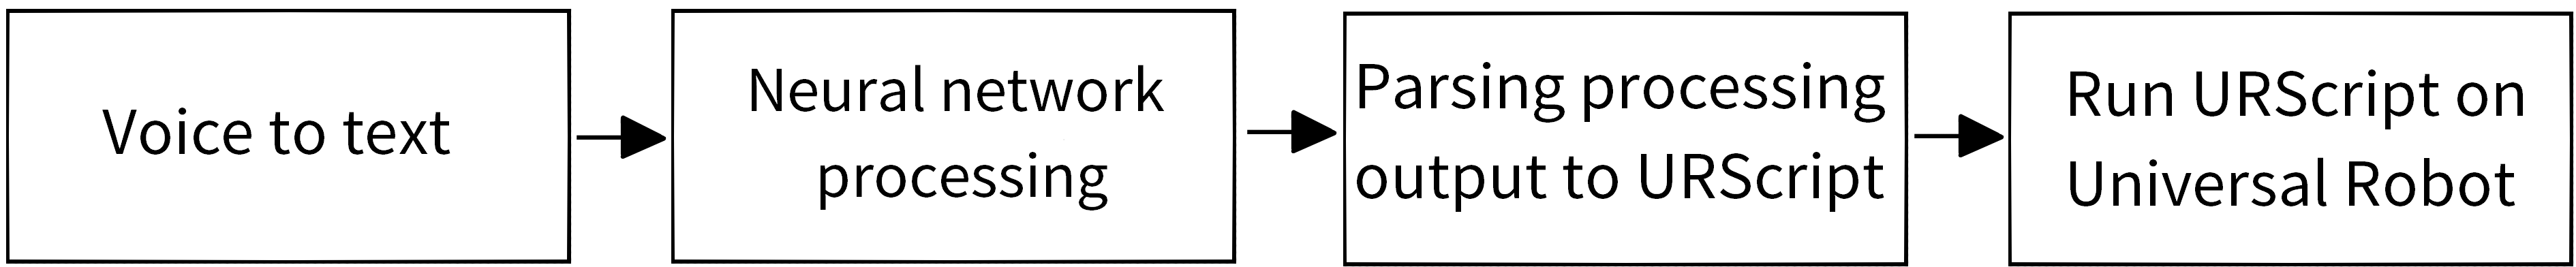
\includegraphics[width=15cm]{img/Picture1.png}
    \caption{Diagram of the work structure}
    \label{Diagram}
\end{figure}



% Commented out the old proposed solution.
\begin{comment} 
    
The task at hand will therefore be designing and training a 
neural network capable of outputting such results.
Afterwards, a parser will be used to analyse the text using a grammatical 
set of rules to identify the commands. Afterwards, the parser 
will build the correct sequence of prewritten UR scripts and send it 
to the robot. 

\vspace{2mm}

For this solution to work, a list of prewritten UR scripts 
must be made. The scripts must be designed such that combinations can 
be used, to theoretically accomodate any legal commands within the 
scope of the project.

\end{comment}




% Commented out the old problem specifying.
\begin{comment}

As the use of natural language processing to control robots, 
is a rather vague problem, some specification and limits must be set.
For the text input of the system. If the input contains a robot command, 
then all actions must either be based on the robots joints, 
or a set of of three points in space, named point A, B and C. These limits set, 
ensures that the commands can be executed contextfree. An example 
for a command which could be done, would be as the following.

\vspace{5mm}
\textit{"move to point A, then move to point B, then move Point 
A 10 centimeters in its z-direction, repeat 5 times."}
\vspace{5mm}

The correct response would be the robot arm zigzagging 5 times 
between point A and point B, where point A would shift slightly 
every time. 

An example of how to robot can be controlled, using itself as a 
reference, could be as follows.

\vspace{5mm}
\textit{"turn joint 1 60 degrees, then turn joint 2 -30 degrees, then 
set point B, to the tool coordinate frame."}
\vspace{5mm}

An example of a command which the robot would not be 
able to execute would be \textit{"stretch}, or \textit{"pose like the 
Letter T"}. As these would require additional contextual information 
that will not be implemented in this project.

\end{comment}





    
    